\chapter{Solução proposta}
\section{Eletrônica}


\subsection{Solução Eletrônica}
O sistema eletrônico tem como objetivo captar a aproximação de veículos ao longo da pista, fazer a detecção de sua velocidade, verificar se a mesma se encontra na faixa permitida pela via, e caso não esteja, capturar a placa do veículo infrator. Uma vez capturada a placa do veículo, o sistema envia a imagem para uma rede remota, onde a mesma fará a identificação. Para isso foi projetado alguns módulos responsáveis por assegurar o funcionamento de todo sistema, apresentados na Fig. \ref{fig:sistemacompleto}.

\begin{figure}[h]
	\center{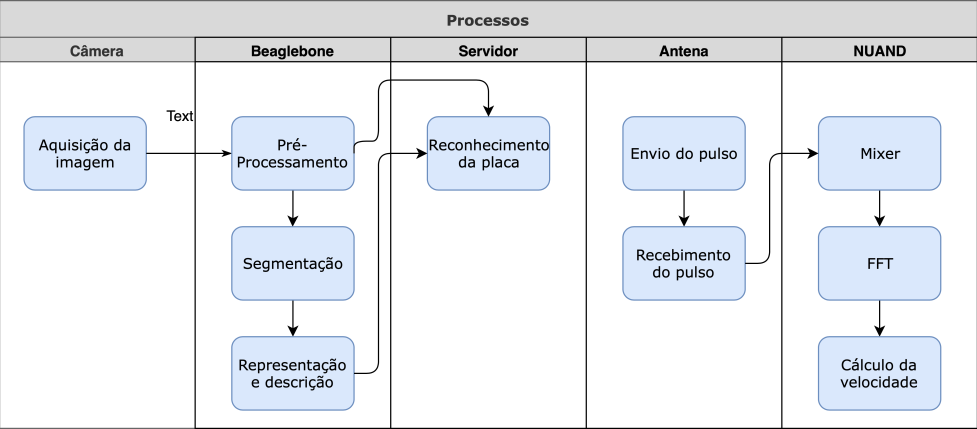
\includegraphics[scale=0.5]{processos-3}}
	\caption{\label{fig:sistemacompleto} Diagrama do sistema eletrônico.}
\end{figure}


\subsubsection{Módulo de aquisição da velocidade}
 O módulo tem como objetivo enviar uma onda modulada na direção do veículo. A partir do fenômeno de refração a mesma irá voltar para antena, entretanto, de acordo com a velocidade do veículo ocorre uma pequena variação na frequência emitida pela antena. De acordo com essa diferença é possível estimar sua velocidade. 


\subsubsection{Módulo Embarcado}

O módulo embarcado dentro da beaglebone tem como função principal servir de centro de operações dos demais componentes ou módulos presente no sistema, de modo que é realizado nele a comparação da velocidade do veículo com a velocidade limite, o pré-processamento da imagem e também a comunicação entre o outro radar localizado no outro extremo da curva e também com o servidor remoto. 

\begin{itemize}
	\item Conferir a velocidade
	\item Capturar a imagem da placa
	\item Receber informação do outro radar para acionar iluminação.
\end{itemize}



\subsubsection{Módulo de reconhecimento do veículo}
 O módulo tem como objetivo realizar a captura e enquadramento de um veículo em uma imagem. Uma vez detectado um automóvel acima da velocidade limite da via a câmera irá realizar o \textit{screenshot} da gravação, onde a imagem logo em seguida passara por um pré-processamento para ser enviada há um servidor remoto, apresentado na Fig. \ref{fig:processos}.
 
 \begin{figure}[!htb]
	\center{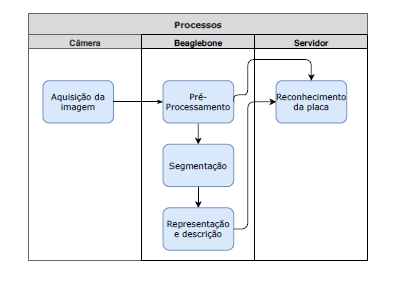
\includegraphics[scale=1]{processos}}
	\caption{\label{fig:processos} Diagrama do sistema do processamento da imagem.}
\end{figure}

 
\subsection{Componentes Eletrônicos}

\subsubsection{Antena}

Responsável pela emissão e detecção dos pulsos eletromagnéticos. Ela enviará uma onda em uma determinada frequência, e recebe essa onda em uma outra frequência determinada pela velocidade do veículo. Ela irá operar na faixa de 915 MHz.

\subsubsection{\emph{Nuand Blade RF x115}}

Na Fig. \ref{fig:nuand}, será apresentado o diagrama de processos entre o \emph{Nuand Blade} e a antena.

 \begin{figure}[!htb]
	\center{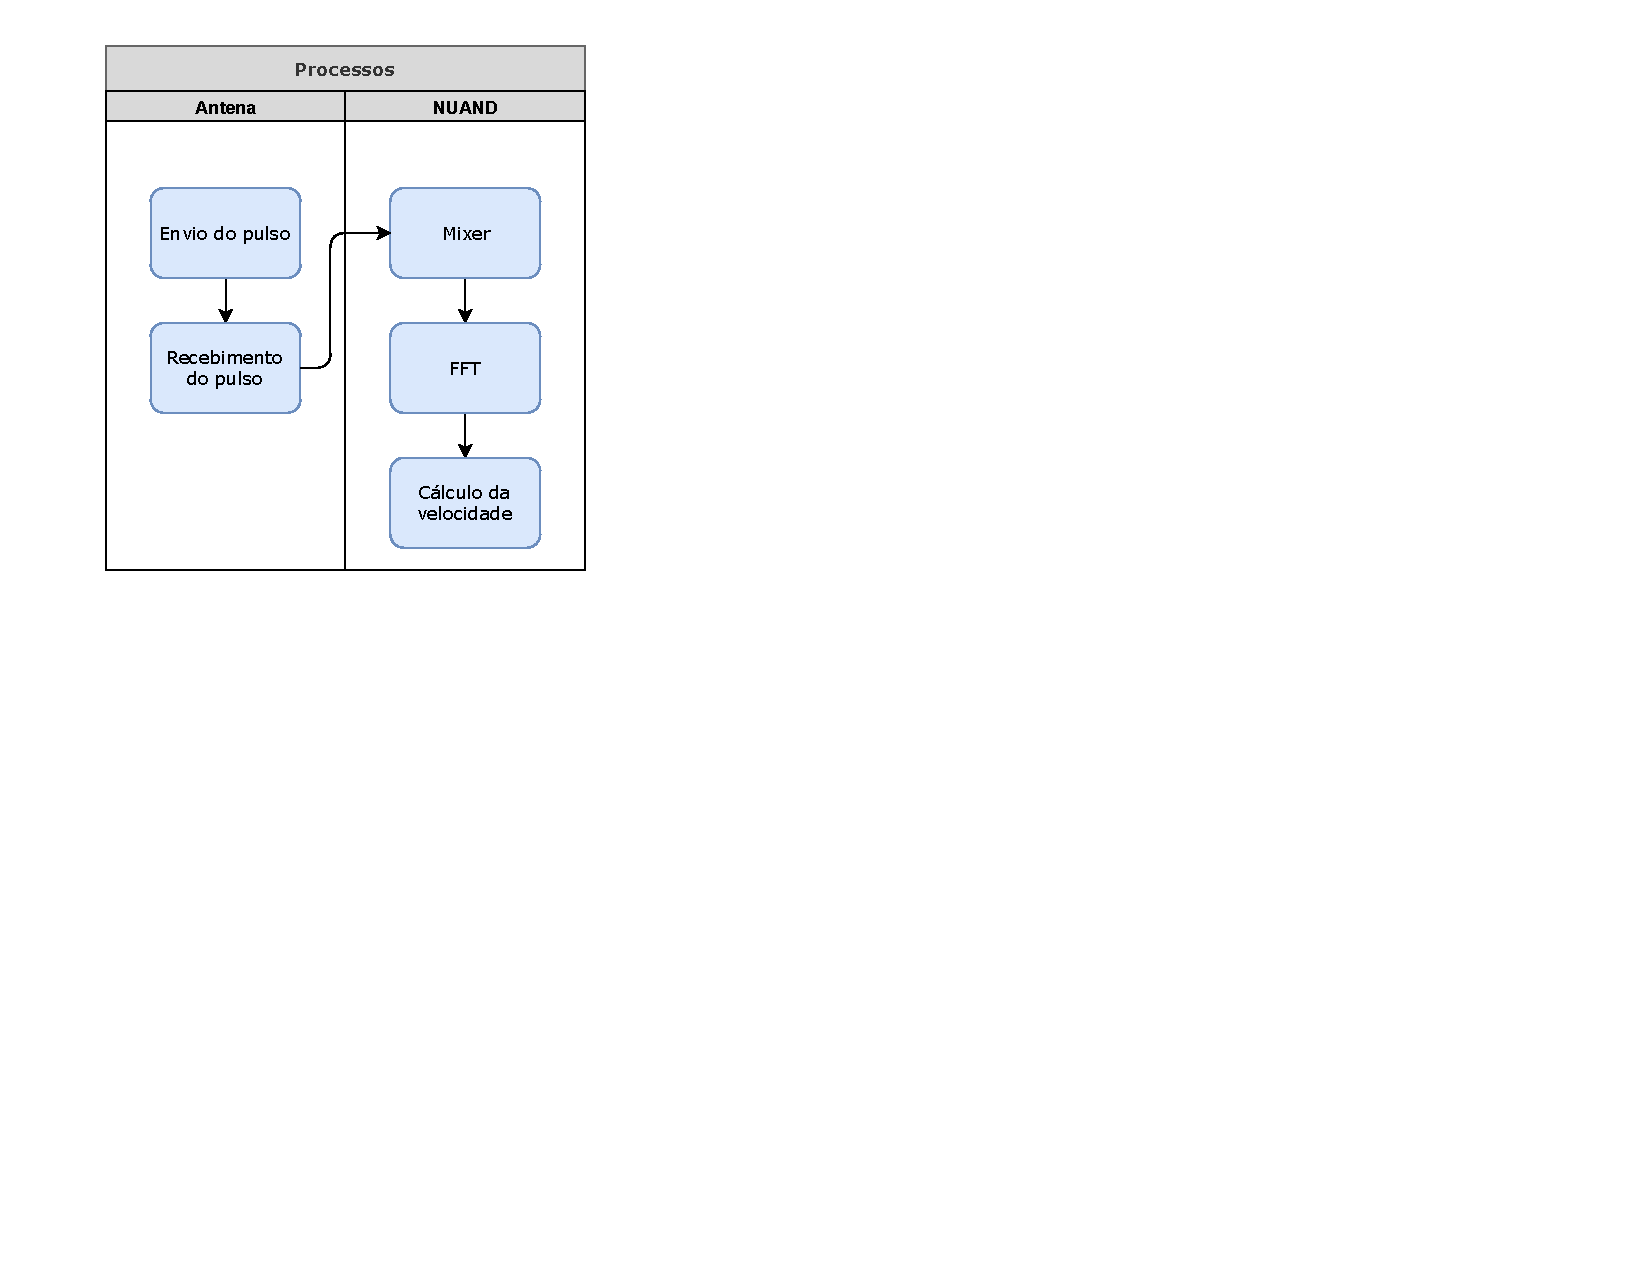
\includegraphics[scale=1]{processos-2}}
	\caption{\label{fig:nuand} Diagrama do sistema do Nuand e antena.}
\end{figure}

De acordo com a Fig. \ref{fig:nuand}, o rádio definido por software será responsável pela modulação do pulso enviado e recebido pela antena. Dentro da placa de desenvolvimento encontra-se um mixer para realização do deslocamento do espectro com o intuito de facilitar a amostragem do sinal. Após o deslocamento é realizado uma filtragem das altas frequências para limpar as possíveis interferências de outros sinais. Após a filtragem é utilizado um algoritmo para realizar a FFT do sinal amostrado e para depois passar por um outro processo onde é possível estimar a sua velocidade, o rádio é apresentado na Fig. \ref{fig:bladerf}. 

\begin{figure}[!htb]
	\center{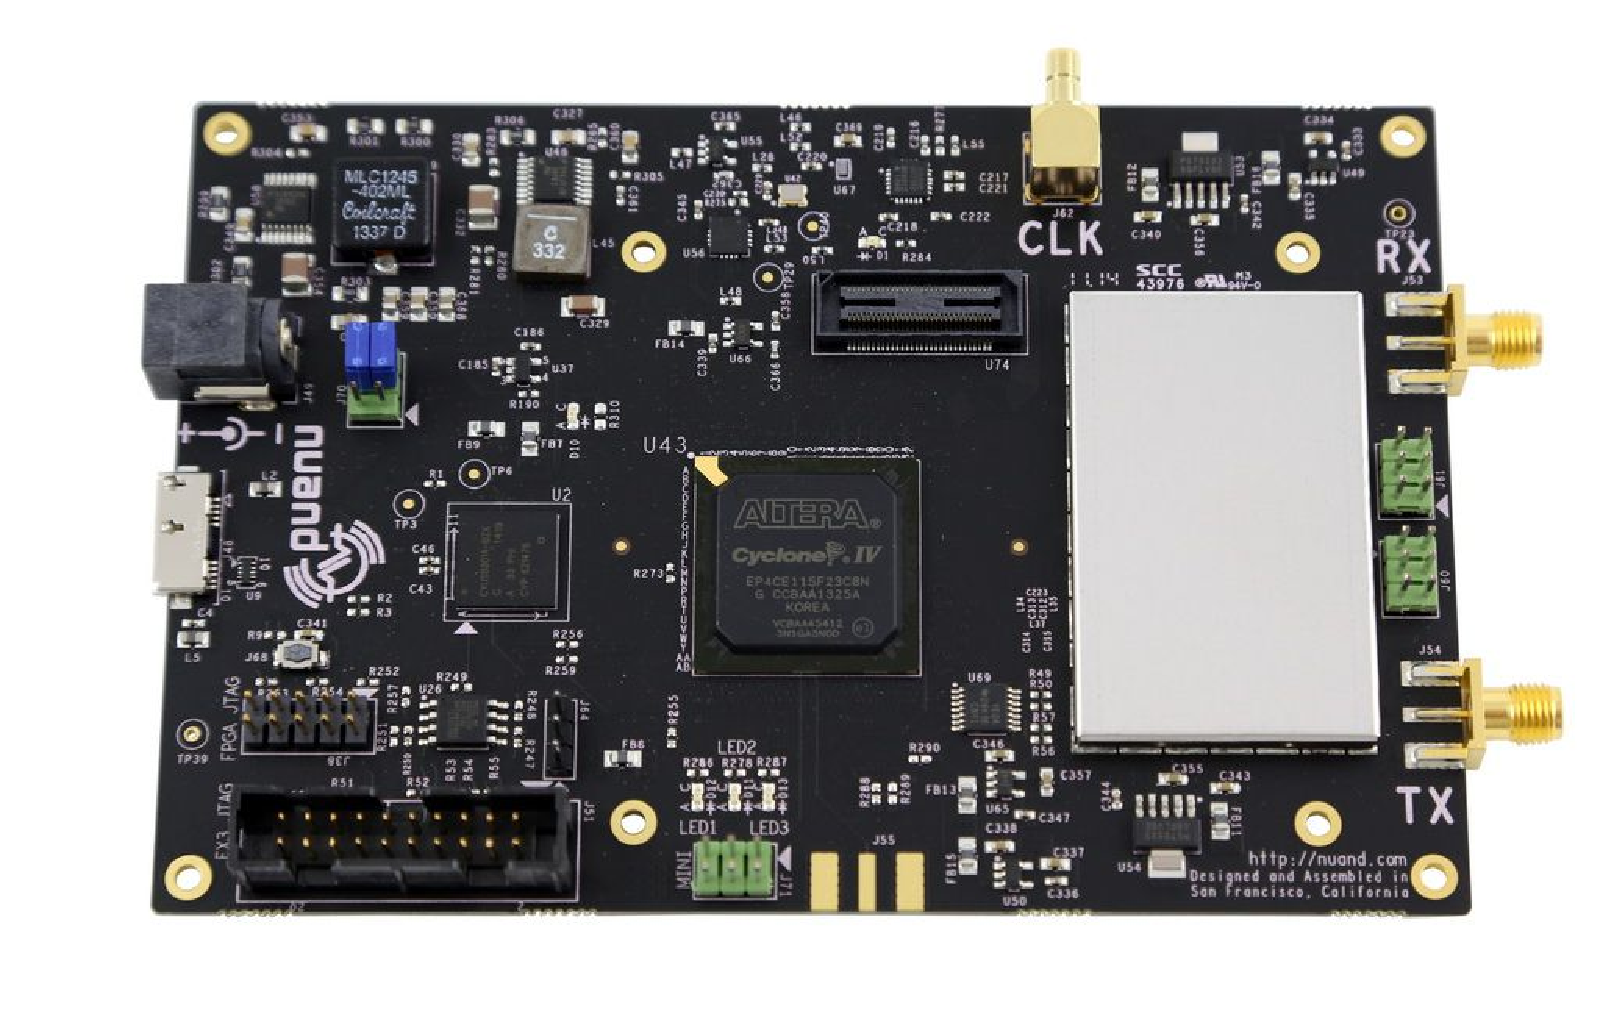
\includegraphics[scale=0.35]{bladerf}}
	\caption{\label{fig:bladerf} Placa BladeRF NUAND}
\end{figure}



\subsubsection{\emph{Beaglebone Black Rev C}} 

A \emph{Beaglebone Black} é um sistema embarcado, como apresentado na Fig. \ref{fig:beaglebone}, que recebe do rádio definido por software \emph{NUAND} a velocidade média do veículo, e a partir deste dado o sistema da \emph{beagle} será responsável por verificar se o mesmo está acima da velocidade permitida da via. Se realmente a velocidade for superior, ela mandará um comando para a câmera para que a mesma realize um \textit{screenshot} de sua gravação para capturar uma imagem do veículo infrator. Após a captura da imagem do automóvel, a \emph{beagle} realizará o pré-processamento, o enquadramento da imagem e aumento ou diminuição do contraste para facilitar o processamento realizado dentro de um servidor. Além disso, a mesma é responsável por todo o controle do sistema de iluminação, que alertará o condutor que existe um veículo se aproximando em direção contrária.

\begin{figure}[!htb]
	\center{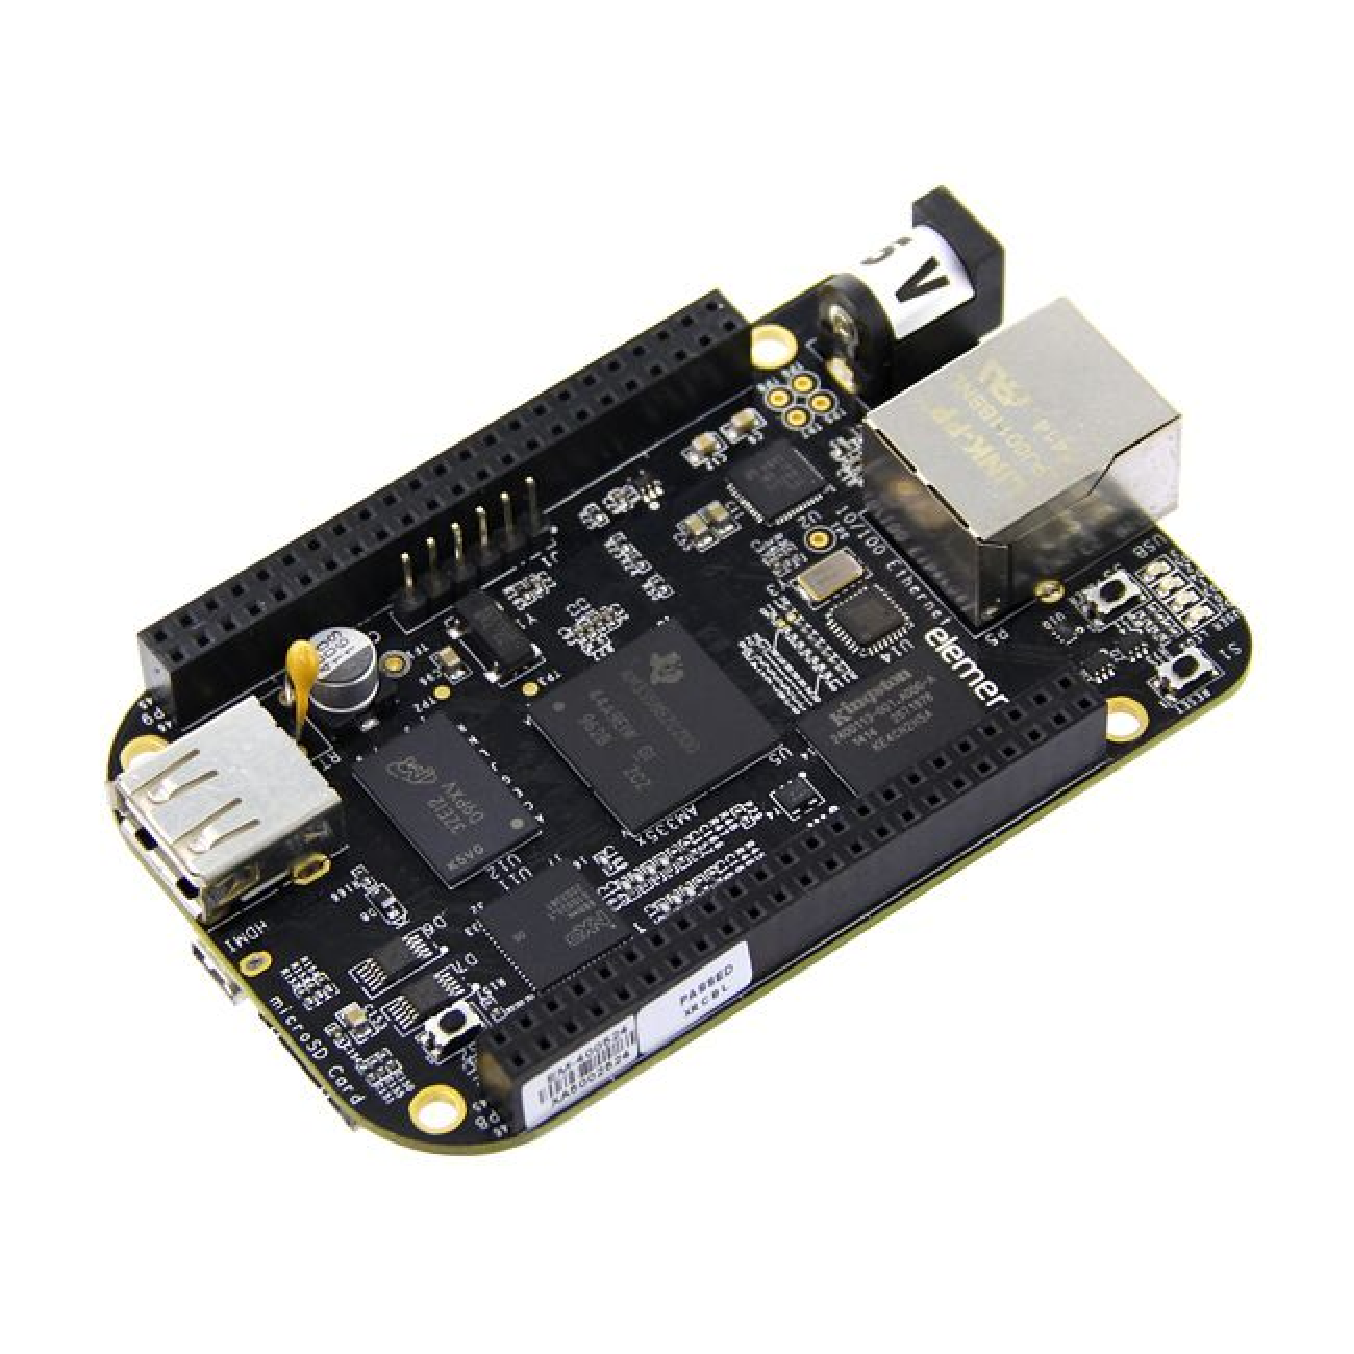
\includegraphics[scale=0.3]{beaglebone}}
	\caption{\label{fig:beaglebone} Sistema embarcado Beaglebone Black}
\end{figure}

\begin{itemize}

\item Especificações do Processador:

– Chip: AM335x 1GHz ARM® Cortex-A8
– Memória: 512MB DDR3 RAM
– Armazenamento: 4GB 8-bit eMMC on-board flash storage
– 3D graphics accelerator
– NEON floating-point accelerator
– 2x PRU 32-bit microcontrollers

\item Interface:
– USB 2.0 Client, para alimentação e comunicação
– USB 2.0 Host
– 10/100M Ethernet (Conector RJ45)
– Interface LCD
– HDMI
– Slot cartão TF
– 2x 46 Pinos

\item  Compatibilidade de Softwares:
– Debian
– Android
– Ubuntu
– Cloud9 IDE em Node.js com biblioteca BoneScript

\item  Especificações Gerais:
– Tensão de operação: 5V/0,35A
– Temperatura de operação: 0-70$^{\circ}$C
– Dimensões: 86,36 x 54,61mm
    
\end{itemize}
 \subsubsection{Módulo \emph{NRF24L10}} 

Tem como função fazer a comunicação entre os dois radares no meio da rodovia. Este módulo foi escolhido pelo fato que o mesmo permite uma boa comunicação sem fio a longas distâncias em lugares abertos, possibilitando assim o envio e a recepção de informações de uma forma simples e rápida de um radar para o outro. A comunicação deste módulo com a placa Beaglebone será pelo protocolo \emph{Serial Peripheral Interface} (SPI), como mostrado na Fig. \ref{fig:nrf24}. 

\begin{figure}[!htb]
	\center{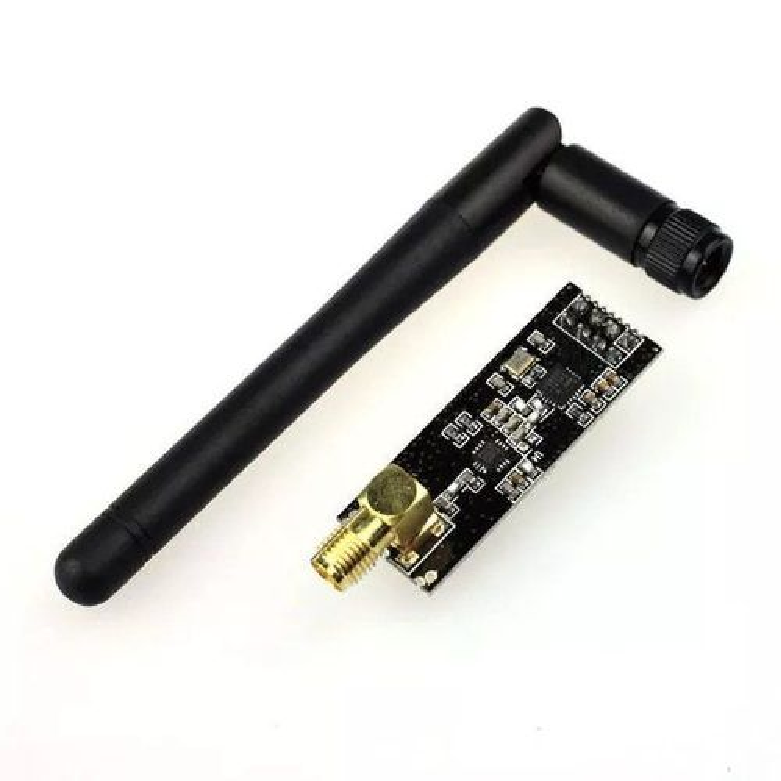
\includegraphics[scale=0.5]{nrf24}}
	\caption{\label{fig:nrf24} Módulo GSM  GPRS}
\end{figure}
\begin{itemize}
    
\item  Especificações:
– Controlador NRF24L01
– Frequência: 2.4GHz
– Tensão de operação: 1.9 à 3.6V
– Taxa de transferência: 2 Mbit/s
– Modulação GFSK
– Regulador de tensão embutido
– Corrente em power down: 400nA
– Corrente em standby: 32uA
– Conector para antena SM
– Dimensões: 29 x 15mm
– Alcance: 1 Km, antena externa.
\end{itemize}

 \subsubsection{Módulo GSM GPRS}
 
Tem como função fazer a comunicação entre os radares e o servidor. Este módulo foi escolhido principalmente pelo fato de apresentar uma ampla disponibilidade de área para conexão e apresenta também uma banda que atende as necessidades de transmissão do projeto, como apresentado na Fig. \ref{fig:gsm}.

 
\begin{figure}[!htb]
	\center{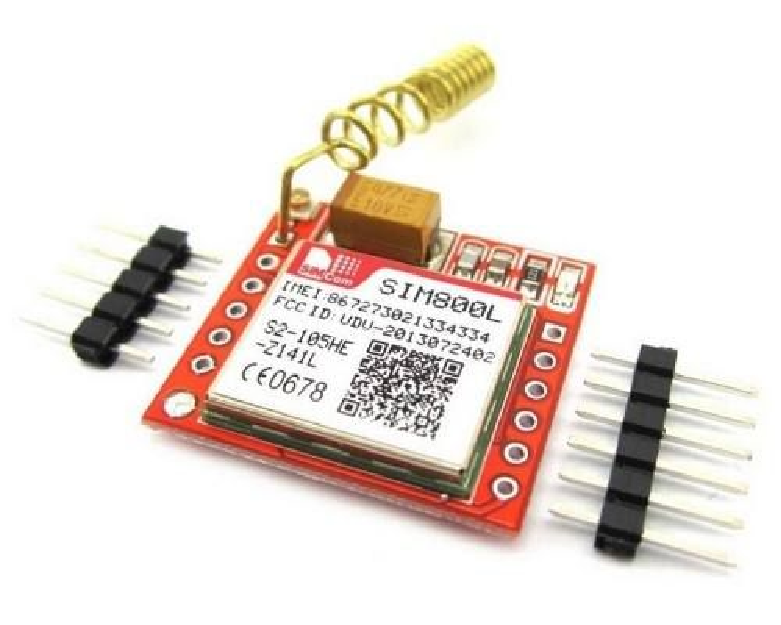
\includegraphics[scale=0.5]{gsm}}
	\caption{\label{fig:gsm} Módulo GSM  GPRS}
\end{figure}

 \begin{itemize}
    
\item Especificações:
–  Tensão de alimentação: 3.7 - 4.2V
– CI SIM800L (datasheet)
– Frequencias: EGSM900, DCS1800, GSM850, PCS1900
– Conector para antena externa U.FL
– GPRS Data Downlink: 85.6 kbps (máximo)
– GPRS Data Uplink: 85.6 kbps (máximo)
– Suporte PAP (password authentication protocol) para conexões PPP
– Protocolo TCP/IP embutido
– Serial: 1200 bps à 115.200 bps
– Slot MicroSIM
– Acompanha antena mola
– Temperatura de operação: -40 a $85^{\circ}C$
– Dimensões: 21 x 15 x 3,2mm
\end{itemize}

\subsubsection{Câmera} 

A câmera tem como função realizar a captura das imagens que serão processadas.  Para que a imagem tenha uma resolução adequada é necessário que a câmera atinja algumas especificações. Dentre elas é necessário que a mesma possua uma lente de pelo menos 6mm para que a mesma possa enxergar com nitidez objetos na faixa de 7-10 metros de distância, outro fator importante é a sensibilidade dos seus sensores de modo que o mais adequado seria que o mesmo possuísse entre 1/2.8"e 1/2"sendo desejado o de 1/2". Esses fatores influenciam no ângulo de abertura da câmera, sendo que quanto menor ele maior a quantidade de informação presente na Fig. \ref{fig:camera}, obtida pela câmera.
\pagebreak

\begin{figure}[!htbp]
    \centering
        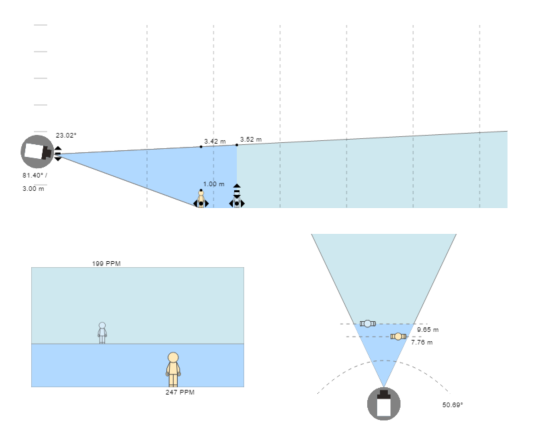
\includegraphics[scale=0.5]{camera.png} 
    \caption{Análise das configurações de uma câmera}
    \label{fig:camera}
\end{figure}

\section{Energia}

Com o objetivo de atender às demandas de energia do projeto, a solução básica adotada foi a utilização de painéis solares em sistemas isolados para geração de energia elétrica, utilizando baterias para a garantia de alimentação em regime permanente e controladores de carga para evitar sobrecargas ou descargas exageradas na bateria, aumentando sua vida útil e desempenho. Também faz parte da solução básica de energia o dimensionamento da iluminação onde serão utilizados painéis e lâmpadas de LED. O sistema, a princípio, tem como objetivo atender a todas as demandas de consumo enérgico dos subsistemas iluminação, aparelhos e componentes eletrônicos, o esquemático do sistema de alimentação é apresentado na Fig. \ref{fig:diagrama_energia}.

\begin{figure}[!htb]
	\center{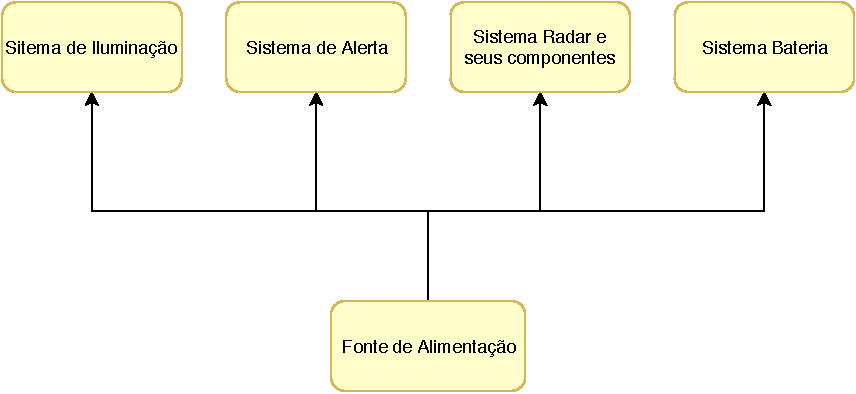
\includegraphics[scale=0.7]{Diagrama_de_Blocos_Energia_2}}
	\caption{\label{fig:diagrama_energia} Diagrama do sistema de alimentação}
\end{figure}

\section{Estrutura}
\section{Software}

\subsection{Detalhamento dos \emph{softwares}}
Radares usados no trânsito das cidades necessitam se comunicar com outros sistemas, tanto para passarem as informações obtidas dos automóveis monitorados quanto dados sobre o próprio funcionamento.

Além disso, é necessário às equipes que darão manutenção aos radares terem condições de obterem dados do funcionamento do sistema deles, para decidirem se e qual intervenção necessitarão fazer no equipamento.

Tendo isso em vista, serão duas soluções em \emph{software} para dar suporte ao funcionamento do radar. O primeiro serviço fará uso de microsserviços para o monitoramento remoto dos radares, já o segundo será uma aplicação a ser usada por equipes de manutenção no diagnóstico dos equipamentos. A Figura \ref{fig:diagrama-in-out-software} mostra o diagrama de como esses softwares interagirão com o radar:

\begin{figure}[!htb]
    \center{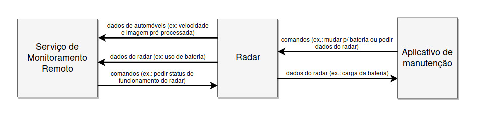
\includegraphics[width=\textwidth]{diagrama-in-out-software}}
    \caption{\label{fig:diagrama-in-out-software} Diagrama de comunicação dos \emph{softwares} com o radar.}
\end{figure}

 A seguir, serão melhor detalhados os \emph{softwares}, assim como suas funcionalidades.

\subsubsection{Serviço de Monitoramento Remoto (SMR)}
Este serviço, que é um dashboard que possui um servidor de microsserviços que dá suporte a ele, terá a função de obter os dados sobre automóveis enviados pelos radares, receber informações sobre o funcionamento dos equipamentos por exemplo, se eles estão com a bateria ou os LEDs funcionando, e a partir disso realizar diversas operações.

As funcionalidades desse serviço serão:

\begin{itemize}
\item{Recepção dos dados dos radares}

Os dados enviados por todos os radares serão recebidos pelo SMR e armazenados no banco de dados.

\item{Processamento de imagens de veículos}

As imagens enviadas pelos radares virão pré-processadas. Caberá ao SMR fazer o restante do processamento delas e, a partir disso, pegar as informações da placa dos automóveis.

\item{Verificação da placa do veículo}

O SMR irá checar todas as placas identificadas para saber se o automóvel fotografado foi furtado. Para isso, o SMR acessará o Sinesp ou outro serviço que permita consultar a situação do veículo.

\item{Notificação de irregularidades às autoridades}

Quando um radar fotografar um veículo furtado ou que ultrapassou a velocidade máxima permitida, o serviço irá mandar os dados do automóvel flagrado para as autoridades competentes, para que elas tomem as medidas cabíveis.

Alguns dos dados que serão enviados são a placa, o dia, o horário e a localização do radar que capturou o veículo.

\item{Notificação de possíveis acidentes}

Quando um radar enviar para o serviço uma notificação de possível acidente no local monitorado por ele, o SMR irá notificar uma central que, através de câmeras, irá confirmar se realmente houve um acidente.

Caso não haja câmeras no local, o serviço irá notificar diretamente os bombeiros mais próximos da região onde fica o radar.

\item{Exibição de dados sobre os radares}

O serviço receberá dados sobre todos os equipamentos que se conectarem com ele, como status de funcionamento e problemas com algum componente.

Essas informações poderão ser visualizadas ou usadas em análises de dados.

\item{Exibição de dados enviados pelos radares sobre veículos}

O serviço armazenará os dados sobre as informações relacionadas à veículos enviadas pelos radares, tais como quantidade de imagens enviadas e número de carros flagrados acima da velocidade permitida.

Essas informações poderão ser visualizadas ou usadas em análises de dados.
\end{itemize}

\subsubsection{Aplicativo de Manutenção}

Esse aplicativo mobile terá como principal objetivo auxiliar as pessoas responsáveis pela manutenção dos radares a diagnosticar como está o funcionamento deles.

As principais funcionalidades dele serão:

\begin{itemize}


\item{Exibição de informações sobre o funcionamento do radar}

Através do aplicativo o responsável pela manutenção poderá saber como está o funcionamento de componentes do radar como, por exemplo, dos LEDs e da bateria.

\item{Alteração da fonte de energia do radar}

Através do aplicativo o responsável pela manutenção poderá mudar a fonte de alimentação do radar para a bateria ou para a fonte de energia externa.

\end{itemize}

\subsection{Documento de Arquitetura}\label{documento-de-arquitetura}

Esta seção se reserva a informar as decisões tomadas pela equipe de \emph{software} enquanto a arquitetura de todos os sistemas que forem construídos.

\subsubsection{Finalidade}\label{finalidade}

Esta seção tem como finalidade apresentar uma visão geral arquitetural
do sistemas que compõe a rede de serviços de \emph{software} para o
\textbf{\emph{RaDop - Radar de Efeito Doppler}}, que será usada como
guia no desenvolvimento do projeto e permitirá um entendimento maior de
todos os componentes integrantes destes sistemas, como um todo, além de
descrever comportamentos, padrões, protocolos de comunicação e demais
informações relacionadas ou correlacionadas. Com o detalhamento da
arquitetura, espera-se, também, deixar explicíta as decisões
arquiteturais realizadas pela equipe.

\subsubsection{Escopo}\label{escopo}

O documento presente abrange três camadas de produtos de \emph{software}
proposto pela equipe de Projeto Integrador 2 na UnB/FGA, sendo eles um
servidor de serviços/microserviços que darão suporte ao Radar de Efeito
Doppler, com serviços de manipulação de dados, processamento de imagens,
tomada de decisões em tempo real, entre outros. A segunda se trata de um
\emph{WebApp} de \emph{Dashboard}, onde estará centralizado grande parte dos dados
providos do Radar com painéis de visualização em tempo real e alguns
dados estatísticos do mesmo. E por fim, o último produto de \emph{software} se
trata de uma aplicação \emph{\emph{mobile}} para auxílio de equipes de
manutenção, com dados e informações sobre o equipamento.

\subsubsection{Definições, Acrônimos e Abreviações}\label{definicoes-acronimos-e-abreviacoes}

\begin{itemize}
\tightlist
\item
  \textbf{RaDop}: Nome comercial do Radar produzido pela equipe de
  Projeto Integrador 2.
\item
  \textbf{UnB}: Universidade de Brasília
\item
  \textbf{FGA}: Faculdade Gama
\item
  \textbf{SMR}: Sistema de Monitoramento Remoto
\end{itemize}

\subsection{Produtos de Software}\label{produtos-de-software}

\subsubsection{Servidor de Microserviços RaDop - SMR}\label{servidor-de-microservicos-radop---smr}

A solução de software proposta para o RaDop será composta de um servidor
de serviços/microserviços para realizar tarefas específicas, esses
serviços serão especialistas em tarefas que serão suportadas pelo RaDop,
dessa forma haverá um sistema central que controlará os demais serviços.
A comunicação se dará via API e requisições HTML com transporte, se
necessário, de arquivos JSON com os dados para execução completa e
correta dos serviços. Vale ressaltar que, para sistemas que comunicam
diretamente com componentes eletrônicos do equipamento, o formato de
comunicação pode ser diferente, mas mantendo-se em protocolos de
comunicação em rede, o que pode alterar o formato de transporte de dados
de JSON para um \emph{encoding} mais simples. Os serviços deverão ser
construídos em \href{https://www.python.org/}{python} e/ou em
\href{https://golang.org/}{Go}, podendo ser atribuído a estes uso de
\emph{frameworks}/ferramentas/tecnologias a serem definidas no andamento
do projeto e posteriormente descritos nesta seção. Detalhes da
arquitetura dos mesmos também serão adicionados a posteriori.

\subsubsection{WebApp Dashboard RaDop}\label{webapp-dashboard-radop}

O WebApp Dashboard RaDop será uma aplicação web desenvolvida a partir do
\emph{framework} \href{https://www.djangoproject.com/}{Django}, o qual é
escrito na linguagem de programação
\href{https://www.python.org/}{python}. O \emph{framework} utiliza por
definição o padrão arquitetural \textbf{MVT}, abreviação para
\emph{model}, \emph{view}, \emph{template}, que é derivada do padrão
arquitetural \textbf{MVC}, \emph{model}, \emph{view}, \emph{controller},
amplamente utilizada para esta finalidade e largamente aceita pela
comunidade produtora de software. De acordo com o \emph{site}
DjangoBook, a parte de \emph{controller}, em Django, é tratada pelo
próprio \emph{framework}. Portanto a \emph{View} do \textbf{MVT}
desempenha um papel próximo, mas não igual ao \emph{controller}.

As camadas desse tipo de arquitetura estão descritas no seguinte
formato, abaixo.

\begin{itemize}



\item{\emph{Model}}\label{model}

É uma representação do banco de dados. Além disso, também inclui
características, relações e outros comportamentos que os dados podem
assumir.

O Django inclui varias ferramentas para automatizar tanto quanto
possível o processo e a manipulação do banco de dados, de forma que o
desenvolvedor não precise se preocupar tanto com o banco de dados, o que
ajuda no foco do desenvolvimento da aplicação de forma mais rápida.

\item{\emph{View}}\label{view}

Estabelece uma ponte entre a \emph{Models} e o \emph{Templates}. Recebe
as requisições do usuário a partir do \emph{template}, acessa o banco de
dados e então retorna a informação solicitada pelo usuário, por meio de
HTML, XML e/ou os erros encontrados.

\item{\emph{Template}}\label{template}

Agrega toda a parte visual que estará visível para os usuários. Inclui
os códigos HTML, CSS, JavaScript, entre outras linguagens que são
utilizadas na apresentação da \emph{View}/\emph{Front-end} ao usuário.

\end{itemize}


\subsubsection{Aplicativo RaDop}\label{aplicativo-radop}

O aplicativo RaDop será uma aplicação \emph{mobile} desenvolvida a partir do
\emph{framework} \href{https://facebook.github.io/react-native/}{React-Native}, construído em cima da
linguagem de programação \href{https://www.javascript.com/}{JavaScript}. O
\emph{React-Native} é o que chamamos de \emph{data-driven}, ou seja, ele não
implementa padrões arquiteturais por padrão, apenas utiliza os dados que
recebe (basicamente as funções recebem os dados e devolvem resultados).
No caso do \emph{React} os dados são o estado da aplicação, as \emph{controllers} são
as funções são os componentes e os resultados são a UI. Dessa forma, a
aplicação é modularizada em \textbf{N} componentes, como dito por Jensen \cite{jensen2018} (podendo ser
\emph{stateless} ou \emph{stateful}), o que torna a aplicação escalável,
robusta e de fácil manutenção.

\begin{itemize}


\item{\emph{Stateless}}\label{stateless}

Neste formato de componente apenas recebe dados de outros componentes
para a sua execução, isso infere que cada uma de suas execuções é
independente, portanto não há conexão entre uma transação e outra. Com
isso o componente não retém dados para si, ou estado de sessões,
propriedades, execuções ou outras informações quaisquer em sua
estrutura.

\item{\emph{Statefull}}\label{statefull}

Neste formato o componente controla o seu próprio estado, ou seja, ele
armazena informações de sua própria execução e subsequentemente, como o
próprio nome diz, do seu estado. Com isso, também, o componente fica
responsável pelo envio dessas informações para outros componentes.

\end{itemize}

\subsection{Requisitos e Restrições Arquiteturais}\label{requisitos-e-restricoes-arquiteturais}

\subsubsection{Servidor de Microserviços RaDop - SMR}\label{req-servidor-de-microservicos-radop---smr}

A Tabela \ref{tab:Servidor de Microserviços RaDop} apresenta as restrições e requisitos dos microservições propostos.

\begin{table}[h]
	\caption{Restrições e Requisitos para a construção dos microsserviços propostos}
	\label{tab:Servidor de Microserviços RaDop}
  \resizebox{\textwidth}{!}{\begin{tabular}{|r|l|}
  \hline
  \textbf{Requisito} & \textbf{Ferramenta/Solução}                                                                                                                                                                                                                                                           \\ \hline
  Linguagem & Python 3.7.3 e Go 1.12                                                                                                                                                                                                                                                                         \\ \hline
  Framework & WebSocket, API Rest e Outros                                                                                                                                                                                                                                                                   \\ \hline
  Segurança & \begin{tabular}[c]{@{}l@{}}Os dados utiizados nos serviços/microsserviços\\ de apoio serão armazenados apenas para\\ auditórias e uso em estatísticas/mining/BI,\\ sendo possível o agendamento da remoção\\  dos mesmos para manter sigilo de dados pessoais,\\ caso necessário.\end{tabular} \\ \hline
  \end{tabular}}
  
\end{table}

\subsubsection{WebApp Dashboard RaDop}\label{req-webapp-dashboard-radop}

A Tabela \ref{tab:WebApp Dashboard RaDop} apresenta as restrições e requisitos para construção do sistema em Django.

\begin{table}[h]
 \caption{Restrições e Requisitos para construção do sistema em Django}
 \label{tab:WebApp Dashboard RaDop}
  \resizebox{\textwidth}{!}{\begin{tabular}{|r|l|}
  \hline
  \textbf{Requisito}  & \textbf{Ferramenta/Solução}                                                                                                                                                                                                                                       \\ \hline
  Linguagem  & Python 3.7.3                                                                                                                                                                                                                                                               \\ \hline
  Framework  & Django 2.1.7                                                                                                                                                                                                                                                               \\ \hline
  Plataforma & Web - Navegadores Google Chrome, Apple Safari e Mozilla Firefox                                                                                                                                                                                                            \\ \hline
  Segurança  & \begin{tabular}[c]{@{}l@{}}Todas as informações dos usuários da dashboard\\ devem ser tratadas em sigilo para que\\ apenas o próprio usuário possa visualizá-las,\\  demais informações não serão\\ armazenadas a fim de manter sigilo de dados\\ dos mesmos.\end{tabular} \\ \hline
  \end{tabular}}
  
\end{table}

\subsubsection{Aplicativo RaDop}\label{req-aplicativo-radop}

A Tabela \ref{tab:app} apresenta as restrições e requisitos para o sistema em React-Native.

\begin{table}[h]
\centering
\caption{Restrições e Requisitos para construção do sistema em React-Native}
\label{tab:app}
  \begin{tabular}{|r|l|}
  \hline
  \textbf{Requisito} & \textbf{Ferramenta/Solução}  \\ \hline
  Linguagem          & JavaScript ES 6              \\ \hline
  Framework          & React-Native 0.59            \\ \hline
  Dependências       & Java Oracle JDK 8 e Node 11+ \\ \hline
  Plataforma         & Mobile - Android 4+          \\ \hline
  \end{tabular}
\end{table}

\subsection{Visão Lógica}\label{visao-logica}

\subsubsection{Serviços RaDop}\label{servicos-radop}

A visão lógica dos serviços do RaDop serão melhor apresentados durante a
execução do projeto devido ao fato da necessidade de cada serviço ser
única não permitir apenas uma representação lógica dos mesmos.

\subsubsection{WebApp Dashboard RaDop}\label{visao-webapp-dashboard-radop}

A visão lógica do WebApp Dashboard está descrita na Figura 2.

\begin{figure}[!htb]
    \center{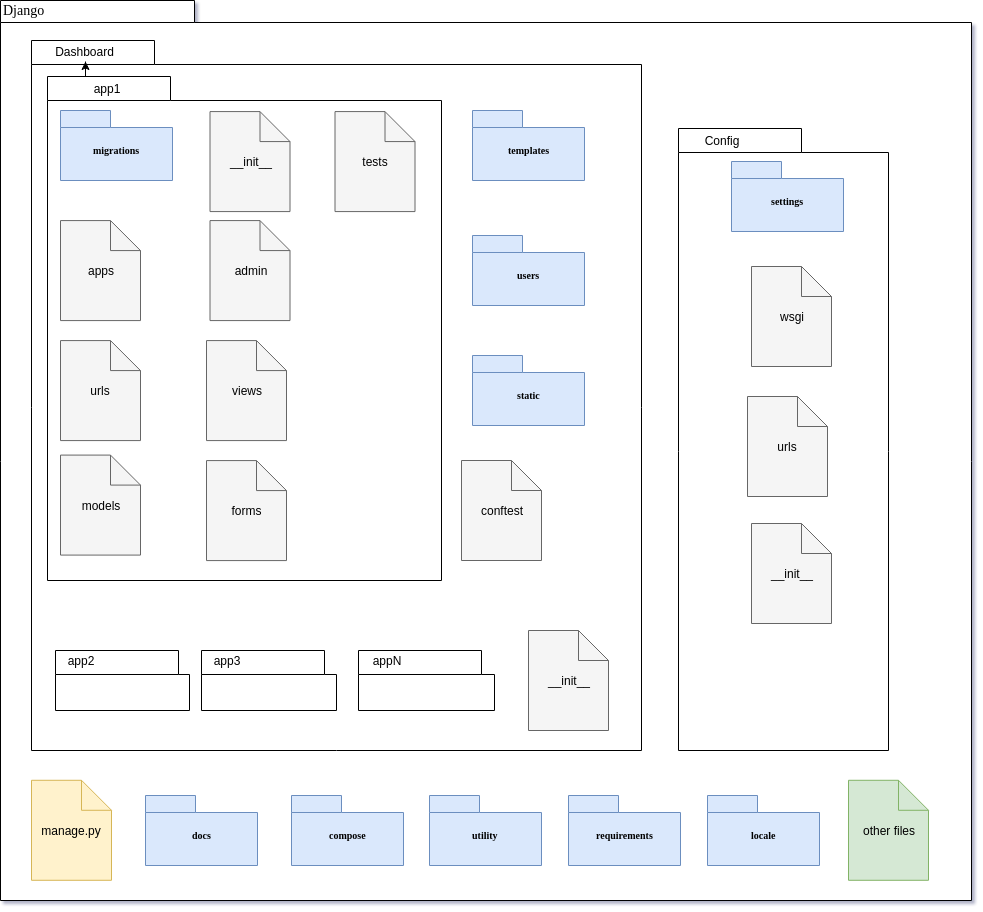
\includegraphics[width=\textwidth]{diagrama-pacotes-django}}
    \caption{\label{fig:diagrama-pact-django} Diagrama de Pacotes Django}
\end{figure}

\subsubsection{Aplicativo RaDop}\label{visao-aplicativo-radop}

A visão lógica do Aplicativo está descrita na Figura 3.

\begin{figure}[!htb]
    \center{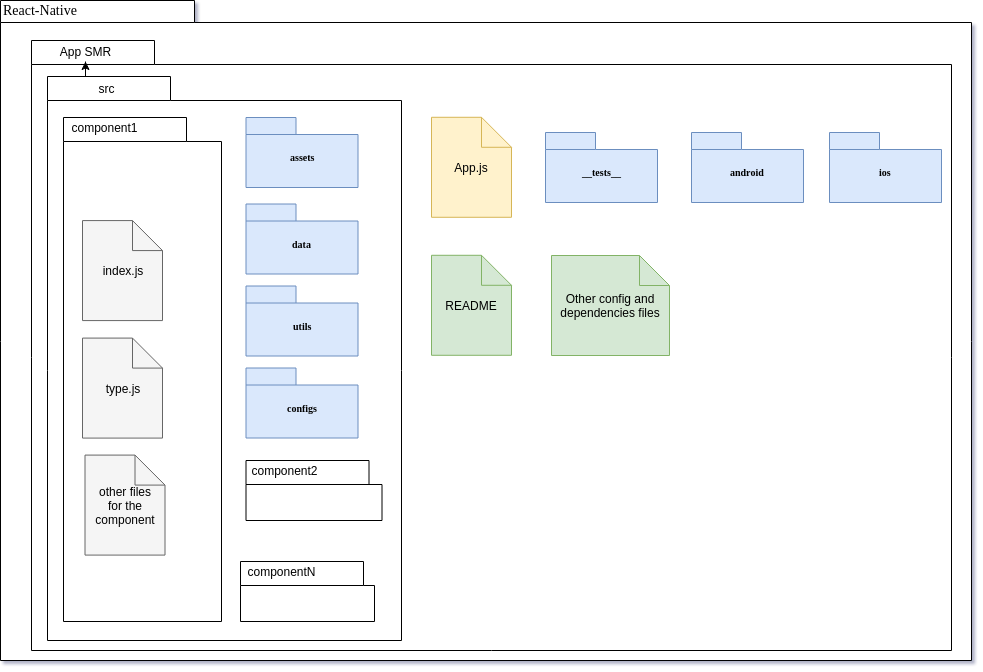
\includegraphics[width=\textwidth]{diagrama-pacotes-react}}
    \caption{\label{fig:diagrama-pact-react}Diagrama de Pacotes React}
\end{figure}

\subsection{Tamanho e Desempenho}\label{tamanho-e-desempenho}

Devido a necessidade de decisões em tempo real os sistemas críticos
deverão ser desenvolvidos de modo a serem o mais perfomáticos possível,
num ponto de vista de tempo de execução, tempo de recebimento de dado e
tempo de envio de dados (excluíndo de fatores externos), e que sejam
capaz de se recuperar de falhas, sejam de redes, de execução e etc. Os
demais sistemas que não forem críticos deverão seguir os melhores
padrões da comunidade produtora de software, afim de manter o seu
tamanho e desempenho dentro de parâmetros aceitáveis pelos
\emph{stakeholders} do projeto.

\subsection{Qualidade}\label{qualidade}

A qualidade das três camadas de produto software para o Radar de Efeito
Doppler - RaDop se darão pelos padrões definidos na comunidade, sendo
avaliado legibilidade de código dado pelo padrão de estilo de escrita,
como o \href{https://www.python.org/dev/peps/pep-0008/}{PEP 8} definido
pelo python, cobertura de código via testes unitários e presença de
testes unitários para funções dos módulos dos sistemas/serviços. As
interfaces visuais serão testadas para serem usáveis, interativas e de
fácil aprendizado, sendo essas validadas com os \emph{stakeholders} do
projeto e com os integrantes da equipe.
